\section{Minimal Motifs: Triangle and Tetrahedron}
\label{sec:motifs}

The smallest instances of $\mathrm{SMN}(n,m)$ occur at $m=2$, where the simplex lattice reduces to the vertices of the simplex alone.  These minimal motifs make the geometry of the architecture fully transparent.

For $(n,m)=(2,2)$, the simplex is the triangle with vertices $a,b,c$, and the hidden nodes are precisely $\{a,c,b\}$.  The input interface is the edge $F_{\mathrm{in}}=\{a,c\}$, the output interface is $F_{\mathrm{out}}=\{c,b\}$, and the shared face is the single point $F_{\mathrm{mid}}=\{c\}$.  The directed hidden edges are $a\to c$, $c\to b$, and $a\to b$, so the motif forms a five-stage feedforward block $i,\,a,\,c,\,b,\,o$ with a skip path from $a$ to $b$.

\begin{figure}[ht]
\centering
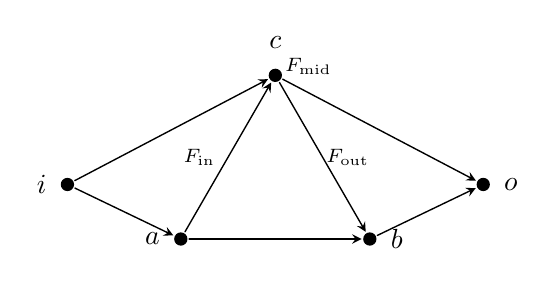
\begin{tikzpicture}[scale=1.2, >=stealth, line width=0.5pt,
                    line cap=round, line join=round]
  % Equilateral triangle: a=(0,0), b=(2,0), c=(1,sqrt(3))
  \coordinate (a) at (0, 0);
  \coordinate (c) at (1, 1.732);
  \coordinate (b) at (2, 0);

  % External nodes (at same height as triangle centroid)
  \coordinate (i) at (-1.2, 0.577);
  \coordinate (o) at (3.2, 0.577);

  % Input connections (to all F_in nodes: a, c)
  \draw[->, shorten <=3pt, shorten >=3pt] (i) -- (a);
  \draw[->, shorten <=3pt, shorten >=3pt] (i) -- (c);

  % Output connections (from all F_out nodes: c, b)
  \draw[->, shorten <=3pt, shorten >=3pt] (c) -- (o);
  \draw[->, shorten <=3pt, shorten >=3pt] (b) -- (o);

  % Hidden edges (DeltaH = 1)
  \draw[->, shorten <=3pt, shorten >=3pt] (a) -- (c);
  \draw[->, shorten <=3pt, shorten >=3pt] (c) -- (b);

  % Skip edge (DeltaH = 2, a to b)
  \draw[->, shorten <=3pt, shorten >=3pt] (a) -- (b);

  % Nodes as solid dots (drawn last, on top of edges)
  \foreach \p in {a, b, c, i, o} \fill (\p) circle (2pt);

  % Labels
  \node[left=4pt]  at (i) {$i$};
  \node[left=4pt]  at (a) {$a$};
  \node[above=6pt] at (c) {$c$};
  \node[right=4pt] at (b) {$b$};
  \node[right=4pt] at (o) {$o$};

  % Facet labels
  \node[left=8pt, font=\scriptsize] at (0.7, 0.866) {$F_{\mathrm{in}}$};
  \node[right=8pt, font=\scriptsize] at (1.2, 0.866) {$F_{\mathrm{out}}$};
  \node[above=8pt, font=\scriptsize] at (1.35, 1.4) {$F_{\mathrm{mid}}$};
\end{tikzpicture}
\caption{Triangle motif $\mathrm{SMN}(2,2)$. Hidden nodes $a,c,b$ with external input $i$ and output $o$. Edges: $i\to a$, $i\to c$ (input injection), $a\to c$, $c\to b$ (single-step), $a\to b$ (skip), $c\to o$, $b\to o$ (readout). Input facet $F_{\mathrm{in}}=\{a,c\}$, output facet $F_{\mathrm{out}}=\{c,b\}$, shared interface $F_{\mathrm{mid}}=\{c\}$.}
\label{fig:triangle-motif}
\end{figure}

The next case, $(n,m)=(3,2)$, gives the tetrahedron motif with vertices $a,b,c,d$.  The hidden nodes are $\{a,c,d,b\}$, the input interface is the face $F_{\mathrm{in}}=\{a,c,d\}$, the output interface is $F_{\mathrm{out}}=\{c,d,b\}$, and the shared face is the edge $F_{\mathrm{mid}}=\{c,d\}$.  The directed hidden edges are $a\to c$, $a\to d$, $c\to b$, $d\to b$, and $a\to b$, yielding a five-stage block $i,\,a,\,\{c,d\},\,b,\,o$ in which the third stage is a parallel two-node layer.

\begin{figure}[ht]
\centering
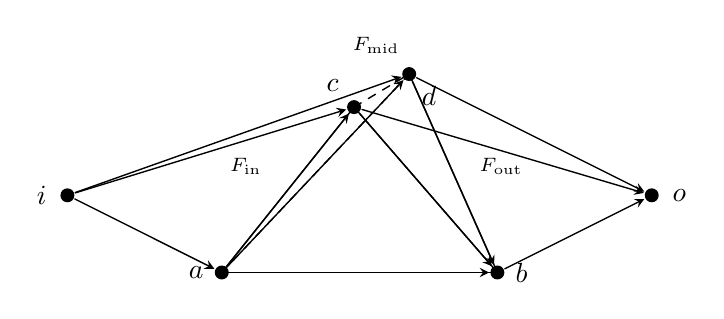
\begin{tikzpicture}[scale=1.4, >=stealth, line width=0.5pt,
                    line cap=round, line join=round]
  % Tetrahedron in perspective projection
  % Base: a (front-left), b (front-right)
  % Top: c (back-left, higher), d (back-right, similar height)
  \coordinate (a) at (0, 0);
  \coordinate (b) at (2.5, 0);
  \coordinate (c) at (1.2, 1.5);
  \coordinate (d) at (1.7, 1.8);

  % External nodes (at average height of vertices)
  \coordinate (i) at (-1.4, 0.7);
  \coordinate (o) at (3.9, 0.7);

  % Tetrahedron edges: back edges dashed (black, same width)
  \draw[dashed] (a) -- (d);      % hidden
  \draw[dashed] (c) -- (d);      % back edge
  \draw (a) -- (b);                        % base
  \draw (a) -- (c);                        % left edge
  \draw (b) -- (c);                        % right edge
  \draw (b) -- (d);                        % right-back edge

  % Input connections (to all F_in nodes: a, c, d)
  \draw[->, shorten <=3pt, shorten >=3pt] (i) -- (a);
  \draw[->, shorten <=3pt, shorten >=3pt] (i) -- (c);
  \draw[->, shorten <=3pt, shorten >=3pt] (i) -- (d);   % to back node

  % Output connections (from all F_out nodes: c, d, b)
  \draw[->, shorten <=3pt, shorten >=3pt] (c) -- (o);
  \draw[->, shorten <=3pt, shorten >=3pt] (d) -- (o);   % from back node
  \draw[->, shorten <=3pt, shorten >=3pt] (b) -- (o);

  % Hidden edges (DeltaH = 1)
  \draw[->, shorten <=3pt, shorten >=3pt] (a) -- (c);
  \draw[->, shorten <=3pt, shorten >=3pt] (a) -- (d);   % to back node
  \draw[->, shorten <=3pt, shorten >=3pt] (c) -- (b);
  \draw[->, shorten <=3pt, shorten >=3pt] (d) -- (b);   % from back node

  % Skip edge (DeltaH = 2, a to b)
  \draw[->, shorten <=3pt, shorten >=3pt] (a) -- (b);

  % Nodes as solid dots (no circles)
  \foreach \p in {a, b, c, d} \fill (\p) circle (1.8pt);
  \foreach \p in {i, o} \fill (\p) circle (1.8pt);

  % Labels
  \node[left=4pt]  at (i) {$i$};
  \node[left=3pt]  at (a) {$a$};
  \node[above left=2pt] at (c) {$c$};
  \node[below right=1pt] at (d) {$d$};
  \node[right=3pt] at (b) {$b$};
  \node[right=4pt] at (o) {$o$};

  % Facet labels
  \node[above left=2pt, font=\scriptsize] at (0.5, 0.75) {$F_{\mathrm{in}}$};
  \node[above right=2pt, font=\scriptsize] at (2.2, 0.75) {$F_{\mathrm{out}}$};
  \node[above=4pt, font=\scriptsize] at (1.4, 1.8) {$F_{\mathrm{mid}}$};
\end{tikzpicture}
\caption{Tetrahedron motif $\mathrm{SMN}(3,2)$. Hidden nodes $a,c,d,b$ with external input $i$ and output $o$. Edges: $i\to a$, $i\to c$, $i\to d$ (input injection), $a\to c$, $a\to d$, $c\to b$, $d\to b$ (single-step), $a\to b$ (skip), $c\to o$, $d\to o$, $b\to o$ (readout). Input facet $F_{\mathrm{in}}=\{a,c,d\}$, output facet $F_{\mathrm{out}}=\{c,d,b\}$, shared interface $F_{\mathrm{mid}}=\{c,d\}$. Dashed edges connect to the back vertex $d$.}
\label{fig:tetrahedron-motif}
\end{figure}

\begin{remark}[MLP-like but not chain-structured]
Both motifs are MLP-like in the sense that they are feedforward, acyclic, and layered. However, they are not ordinary chain-structured MLPs. Instead, they contain geometrically induced parallel channels and skip paths, and their input and output layers are attached to entire faces rather than to a single chain of hidden layers.
\end{remark}
